\chapter{Stokes' Theorem}

\section{Integrating Forms over Parametrized-Manifolds}
\begin{definition}
    Let $A$ be open in $\R^k$. Let $\eta$ be a k-form defined in $A$. Then $\eta$ can be written uniquely in the form 
    $$\eta =f\cdot dx_1\wedge \cdots \wedge dx_k$$
    We define the \underline{integral of $\eta$ over $A$} by the equation $$\int_A\eta=\int_Af$$
    provided that the latter integral exists.
\end{definition}
\noindent\textbf{Remark}:
\begin{itemize}
    \item Forms are more abstract, the integral of forms are even more abstract. But no worries, we will get some geometric intepretation later.
\end{itemize}

\begin{theorem}
    Let $\{a_1,\cdots,a_k\}$ be any right-handed orthonormal basis for $\R^k$, then we have 
    $$\int_A\eta=\int_{x\in A}\eta(x)((x;a_1),\cdots,(x;a_k))$$
\end{theorem}

\begin{definition}
    Let $A$ be open in $\R^k$. Let $\alpha:A\longrightarrow\R^n$ be of class $C^{\infty}$. 
    The set $Y=\alpha(A)$, together with the map $\alpha$, constitute the parametrized-manifold $Y_{\alpha}$. 
    Let $\omega$ be a k-form defined in an open set of $\R^n$ containing $Y$, we define the \underline{integral of $\omega$ over $Y_{\alpha}$} by the equation 
    $$\int_{Y_{\alpha}}\omega=\int_A\alpha^*\omega$$
    provided the latter exists. Since $\alpha^*$ and $\int_A$ are linear, so is this integral.
    $$\int_{Y_{\alpha}}(a\omega+b\eta)=a\int_{Y_{\alpha}}\omega+b\int_{Y_{\alpha}}\eta$$
\end{definition}

\begin{theorem}[Invariant under reparametrization]
    Let $g:A\longrightarrow B$ be a diffeomorphism of open sets in $\R^k$. 
    Assume $\det(Dg)$ does not change sign on $A$. 
    Let $\beta:B\longrightarrow\R^n$ be a map of class $C^{\infty}$. 
    Let $Y=\beta(B)$. Let $\alpha=\beta\circ g$, then $\alpha:A\longrightarrow\R^n$ and $Y=\alpha(A)$. 
    If $\omega$ is a k-form defined in an open set of $\R^n$ containing $Y$, then $\omega$ is integrable over $Y_{\beta}$ if and only if it is integrable over $Y_{\alpha}$. In this case 
    $$\int_{Y_{\alpha}}\omega=\pm \int_{Y_{\beta}}\omega$$
    where the sign agrees with the sign of $\det(Dg)$.
\end{theorem}
\noindent\textbf{Remark}:
\begin{itemize}
    \item If $A$ is connected, then the hypothesis that $\det(Dg)$ does not change sign on $A$ is automatically satisfied.
\end{itemize}

\begin{theorem}
    Let $A$ be open in $\R^k$. Let $\alpha:A\longrightarrow\R^n$ be of class $C^{\infty}$. 
    Let $Y=\alpha(A)$. Let $x$ denote the general point of $A$ and $z$ denote the general point of $\R^n$. If $$\omega=f\cdot dz_I$$
    is a k-form defined in an open set of $\R^n$ containing $Y$, then $$\int_{Y_{\alpha}}\omega=\int_A(f\circ \alpha)\det(\frac{\partial \alpha_I}{\partial x})$$
\end{theorem}

\noindent\textbf{Remark}:
\begin{itemize}
    \item Recall in single-variable calculus. Let $A=(a,b)$ an open interval. Then $$\int_Afdx=\int_a^bf$$
    where the notation $fdx$ on the left denotes the integral of a 1-form and the notation on the right denotes the integral of a function.
\end{itemize}

\section{Orientable Manifolds}

\subsection{Definition of Orientation of Manifolds}

\begin{definition}
    The \underline{support of a differential form}, including a k-form $\omega$, is a concept from the field of differential geometry that describes the region where the form is non-zero. In more precise terms, the support of a k-form $\omega$, denoted as $supp(\omega)$, is the closure of the set of points in the k-manifold $M$ where the form does not vanish:
    $$supp(\omega)=\overline{\{p\in M: \omega(p)\neq 0}\}$$
\end{definition}

\noindent\textbf{Remark}:
\begin{itemize}
    \item To say that $\omega(p)$ does not vanish at a point $p$ means that it is not the zero tensor at that point. In other words, there exists a set of k linearly independent tangent vectors at point $p$ such that the k-tensor $\omega(p)$ evaluated on these vectors is non-zero:
    $$\omega(p)((p;v_1),\cdots,(p;v_k))\neq 0$$
    \item We will define the integral of a k-form $\omega$ over k-manifold $M$ in much the same way that we define the integral of a scalar function over $M$. first we treat the case where the support of $\omega$ lies in a single coordinate patch $\alpha:U\longrightarrow V$. in this case we define
    $$\int_M\omega=\int_{Int(U)}\alpha^*\omega$$
    However, if we change the parametrization of the manifold (i.e., change the coordinate system or the way the manifold is described), the integral's value may change in sign but not in magnitude.
    \item In order to make this well defined, we need an extra condition on $M$, called orientability.
\end{itemize}

\begin{definition}
    In previous section, we defined what is orientation-preserving for linear transformation $h\in \mathcal{L}(\R^k,\R^k)$. 
    We now generalize this to diffeomorphism $g:A\longrightarrow B$ of open sets in $\R^k$.
    \begin{itemize}
        \item We say that $g$ is \underline{orientation-preserving} if $\det(Dg)>0$ on $A$.
        \item We say that $g$ is \underline{orientation-reversing} if $\det(Dg)<0$ on $A$.
    \end{itemize}
\end{definition}

\begin{theorem*}
    Given diffeomorphism $g$, for each point $x\in A$, we have an induced linear transformation on tangent spaces $$g_*:\mathcal{T}_x(\R^k)\longrightarrow\mathcal{T}_{g(x)}(\R^k)$$
    The diffeomorphism $g$ is orientation-preserving if and only if $g_*$ is orientation-preserving in the linear transformation sense for each $x\in A$.
\end{theorem*}

\begin{definition}
    Let $M$ be a k-manifold in $\R^n$. Given coordinate pathches $$\alpha_0:U_0\longrightarrow V_0$$
    $$\alpha_1:U_1\longrightarrow V_1$$
    We say two coordinate pathces \underline{overlap} if $V_0\cap V_1\neq \emptyset$. 
    We say they \underline{overlap positively} if the transition function $$\alpha_1^{-1}\circ \alpha_0:W_0\subset \R^k\longrightarrow W_1$$
    is orientation-preserving.
\end{definition}

\begin{definition}
    If $M$ can be covered by coordinate pathces (also called atlas or charts) $\{(U_i,\alpha_i)\}$ that each pair of which overlap positively(if they overlap), then $M$ is said to be \underline{orientable}. 
    Otherwise, $M$ is said to be \underline{non-orientable}.
\end{definition}

\begin{definition}
    Suppose $M$ is orientable. Given two collection of coordinate pathces $\{(U_i,\alpha_i)\}_{i\in I}$ and $\{(U_j,\alpha_j)\}_{j\in J}$, we can show the union of them is also overlap positively. 
    We put all possible collection of such coordinate patches together, this is called an \underline{orientation} on $M$. 
    A manifold $M$ together with an orientation is called an \underline{oriented manifold}.
\end{definition}
\noindent\textbf{Remark}:
\begin{itemize}
    \item A k-manifold($k\geq1$) can have different orientations. But for 0-manifold, which is a collection of discrete points, this definition makes no sense, we will discuss the orientation of 0-manifold later.
    \item Let $\R^k$ be a vector space of dimension $k$, then $\R^k$ is also a k-manifold. We now have two notions of orientation of $\R^k$. 
    \begin{itemize}
        \item For $\R^k$ as a vector space, it has two orientations. One is the collection of all right-handed k-frames and the other is the collection of all left-handed k-frames.
        \item For $\R^k$ as a k-manifold, it still has two orentations that corresponds to the above two. The connection is easy to describe. Given an orientation of $\R^k$ in the sense of vector space, we can pick a k-frame $(v_1,\cdots,v_k)$. The linear isomorphism $\alpha:\R^k\longrightarrow\R^k$ such that $\alpha(e_i)=v_i$ is a coordinate patch on $\R^k$. And we can check that two coordinate pathces overlap positively.
    \end{itemize}
\end{itemize}

\subsection{Oriented Manifolds in $\R^n$ of Specific Dimension}

\begin{definition}
    Let $M$ be an oriented 1-manifold in $\R^n$. We define a corresponding unit tangent vector field $$T:M\longrightarrow\mathcal{T}(M)$$
    as follows: Given $p\in M$, choose a coordinate patch $\alpha:U\longrightarrow V$ on $M$ about $p$ belonging to the given orientation, we define $$T(p)=(p;\frac{D\alpha(t_0)}{\norm{D\alpha(t_0)}})$$
    where $t_0$ is the parameter value such that $\alpha(t_0)=p$.\\
    Then $T$ is called the \underline{unit tangent field corresponding to the orientation of $M$}.
\end{definition}

\noindent\textbf{Remark}:
\begin{itemize}
    \item The unit tangent field $T$ is the geometric interpretation of the orientation of a 1-manifold.
\end{itemize}

\begin{definition}
    In the case of a 1-manifold $M$, we shall allow the domains of coordinate patches on $M$ to be open sets in $\R^1$ or in $\HH^1$ or in $\mathbb{L}^1$. Where $$\mathbb{L}^1=(-\infty,0]$$
    We will explain why we add $\mathbb{L}^1$ in the following examples.
\end{definition}

\noindent\textbf{Example}:
\begin{itemize}
    \item Given an oriented 1-manifold $M$ without boundary, with corresponding unit tangent field $T$. $M$ has some kind of circular structure, although it can has knots but we do not care here, see the following picture. 
    We often picture the direction of $T$ by drawing an arrow on the curve $M$ itself. 
    \begin{figure}[H]
        \centering
        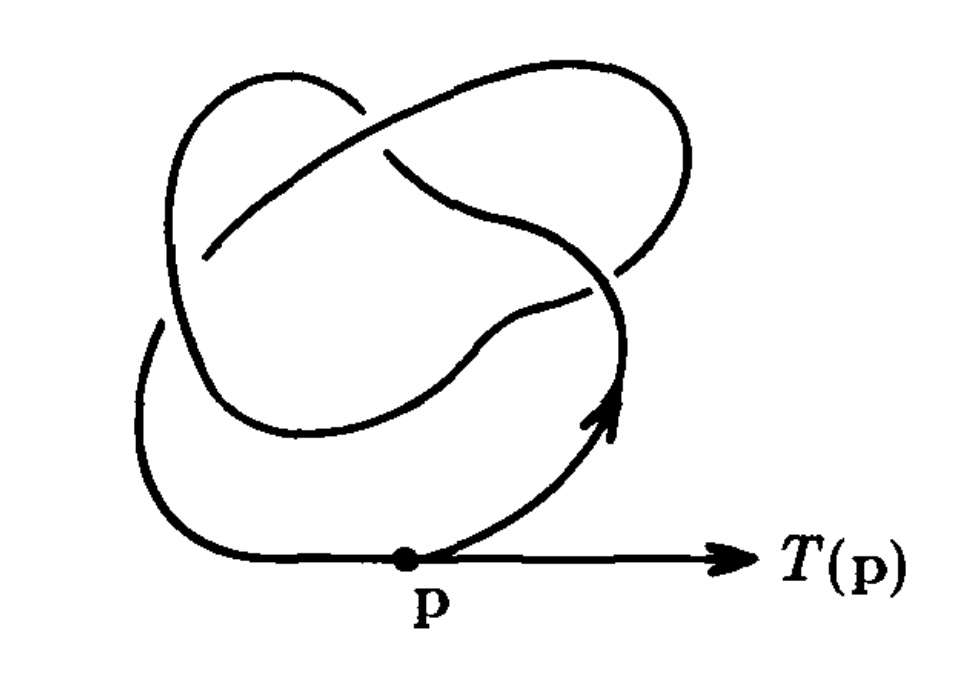
\includegraphics[scale=0.3]{images/Screenshot 2023-04-01 at 17.55.10.png}
    \end{figure}
    \item Now consider an oriented 1-manifold $M$ that has boundary. For the 1-manifomd in the picture, $\partial M$ consists of two points $p$ and $q$. Consider the coordinate pathches about $p$, $q$ respectively $$\alpha:U_1\longrightarrow V_1$$ $$\beta:U_2\longrightarrow V_2$$
    The fact that $U_1$ is open in $\HH^1$ means that the corresponding unit tangent field vector $T(p)$ must points into $M$ form $p$. Similarly, $T(q)$ points into $M$ from $q$. This violates the definition of $T$ because the orientation is messed up. 
    \begin{figure}[H]
        \centering
        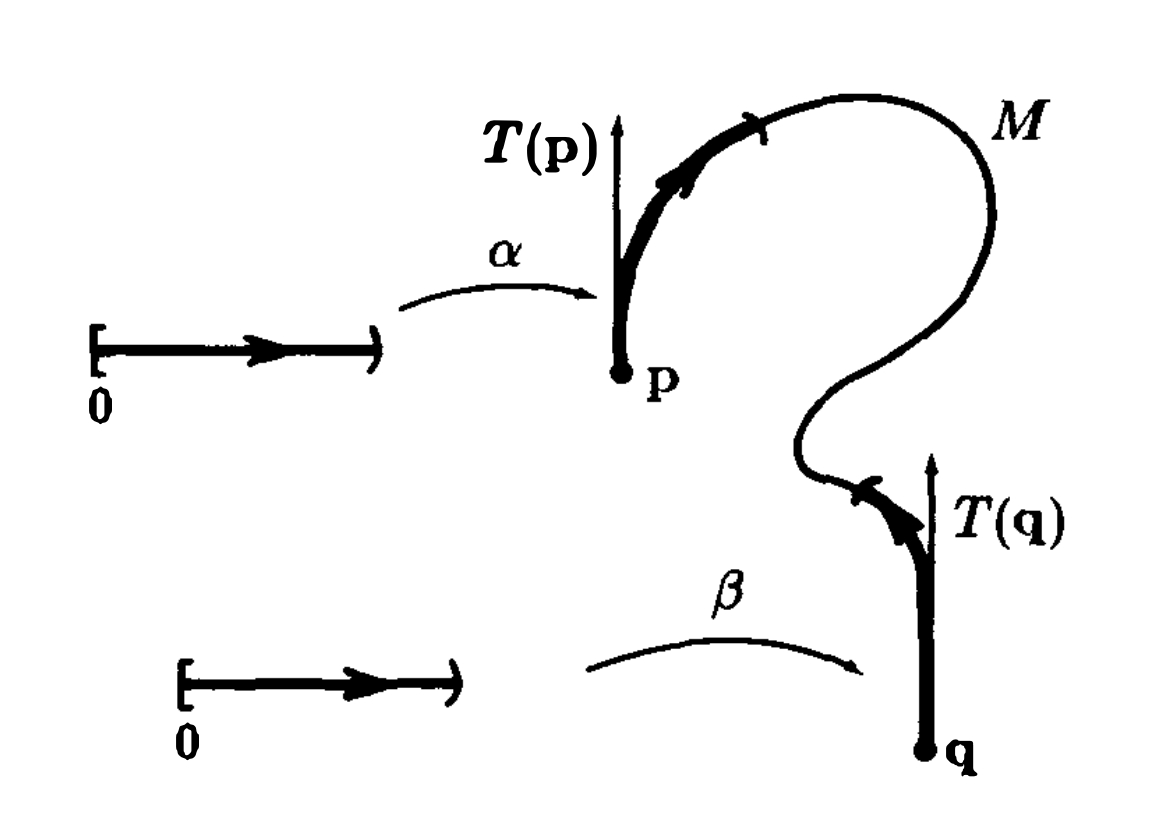
\includegraphics[scale=0.3]{images/Screenshot 2023-04-01 at 18.03.45.png}
    \end{figure}
    The problem disappears if we allow $U_2$ be open in $\mathbb{L}^1$. with this extra degree of freedom, it is easy to cover $M$ by coordinate patches that overlap positively. 
    \begin{figure}[H]
        \centering
        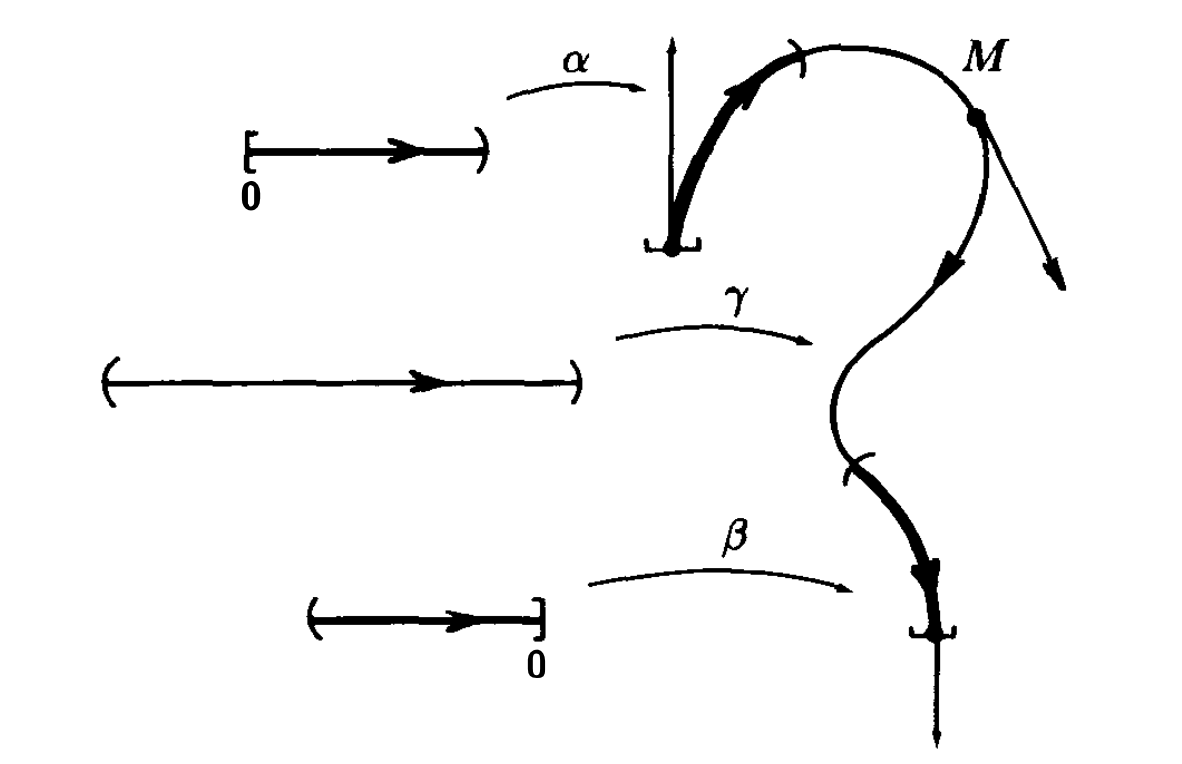
\includegraphics[scale=0.35]{images/Screenshot 2023-04-01 at 18.06.26.png}
    \end{figure}
\end{itemize}

\begin{theorem*}
    With this extra degree of freedom, every 1-manifold is orientable.
\end{theorem*}

\noindent\textbf{Remark}:
\begin{itemize}
    \item We now consider an arbitrary 1-manifold $M$ in $\R^n$. From basic topology, we can partition $M$ into connected components. We consider each component.
    \item If the component has no boundary, it looks like the first example. It has 2 orientations, one is cosidered to be like clockwise and the other is like counterclockwise.
    \item If the component has non-empty boundary, it looks like the second example. It also has 2 orientations, one is considered to be like going forward, and the other is like going backward.
    \item If 1-manifold $M$ has $k$ connected components, then it has $2^k$ orientations.
\end{itemize}

\begin{definition}
    Let $M$ be an (n-1)-manifold in $\R^n$. If $p\in M$, let $(p;n)$ be a unit vector in the n-dimensional vector space $\mathcal{T}_p(\R^n)$ that is orthogonal to the n-1 dimensional linear subspace $\mathcal{T}_p(M)$. 
    Then $n$ is uniquely determined up to sign. Given an orientation of $M$, choose a coordinate patch $\alpha:U\longrightarrow V$ on $M$ about $p$ belonging to this orientation. Let $\alpha(x)=p$. Then the columns $\frac{\partial \alpha}{\partial x_i}$ of the matrix $D\alpha(x)$ give a basis 
    $$\{(p;\frac{\partial \alpha}{\partial x_1}),\cdots,(p;\frac{\partial \alpha}{\partial x_{n-1}})\}$$
    for the tangent space to $M$ at $p$. We specify the sign of $n$ by requiring that the frame $$(n,\frac{\partial \alpha}{\partial x_1},\cdots,\frac{\partial \alpha}{\partial x_{n-1}})$$ be right-handed, that is, the matrix \begin{equation*}
        \begin{bmatrix}
            n & D\alpha(x)
        \end{bmatrix}
    \end{equation*}
    has positive determinant. $n$ is well-defined because we can show it is independent of the choice of $\alpha$. We can view $n$ as a function
    $$n:M\longrightarrow \R^n$$
    We can show that this function $n(p)$ is of class $C^{\infty}$. The vector field $$N(p)=(p;n(p))$$
    is called the \underline{unit normal field to $M$ corresponding to the orientation of $M$}.
\end{definition}

\noindent\textbf{Example}:
\begin{itemize}
    \item Consider the 2-manifold with boundary in $\R^3$ that looks like a weired bell which we saw before.
    \begin{figure}[H]
        \centering
        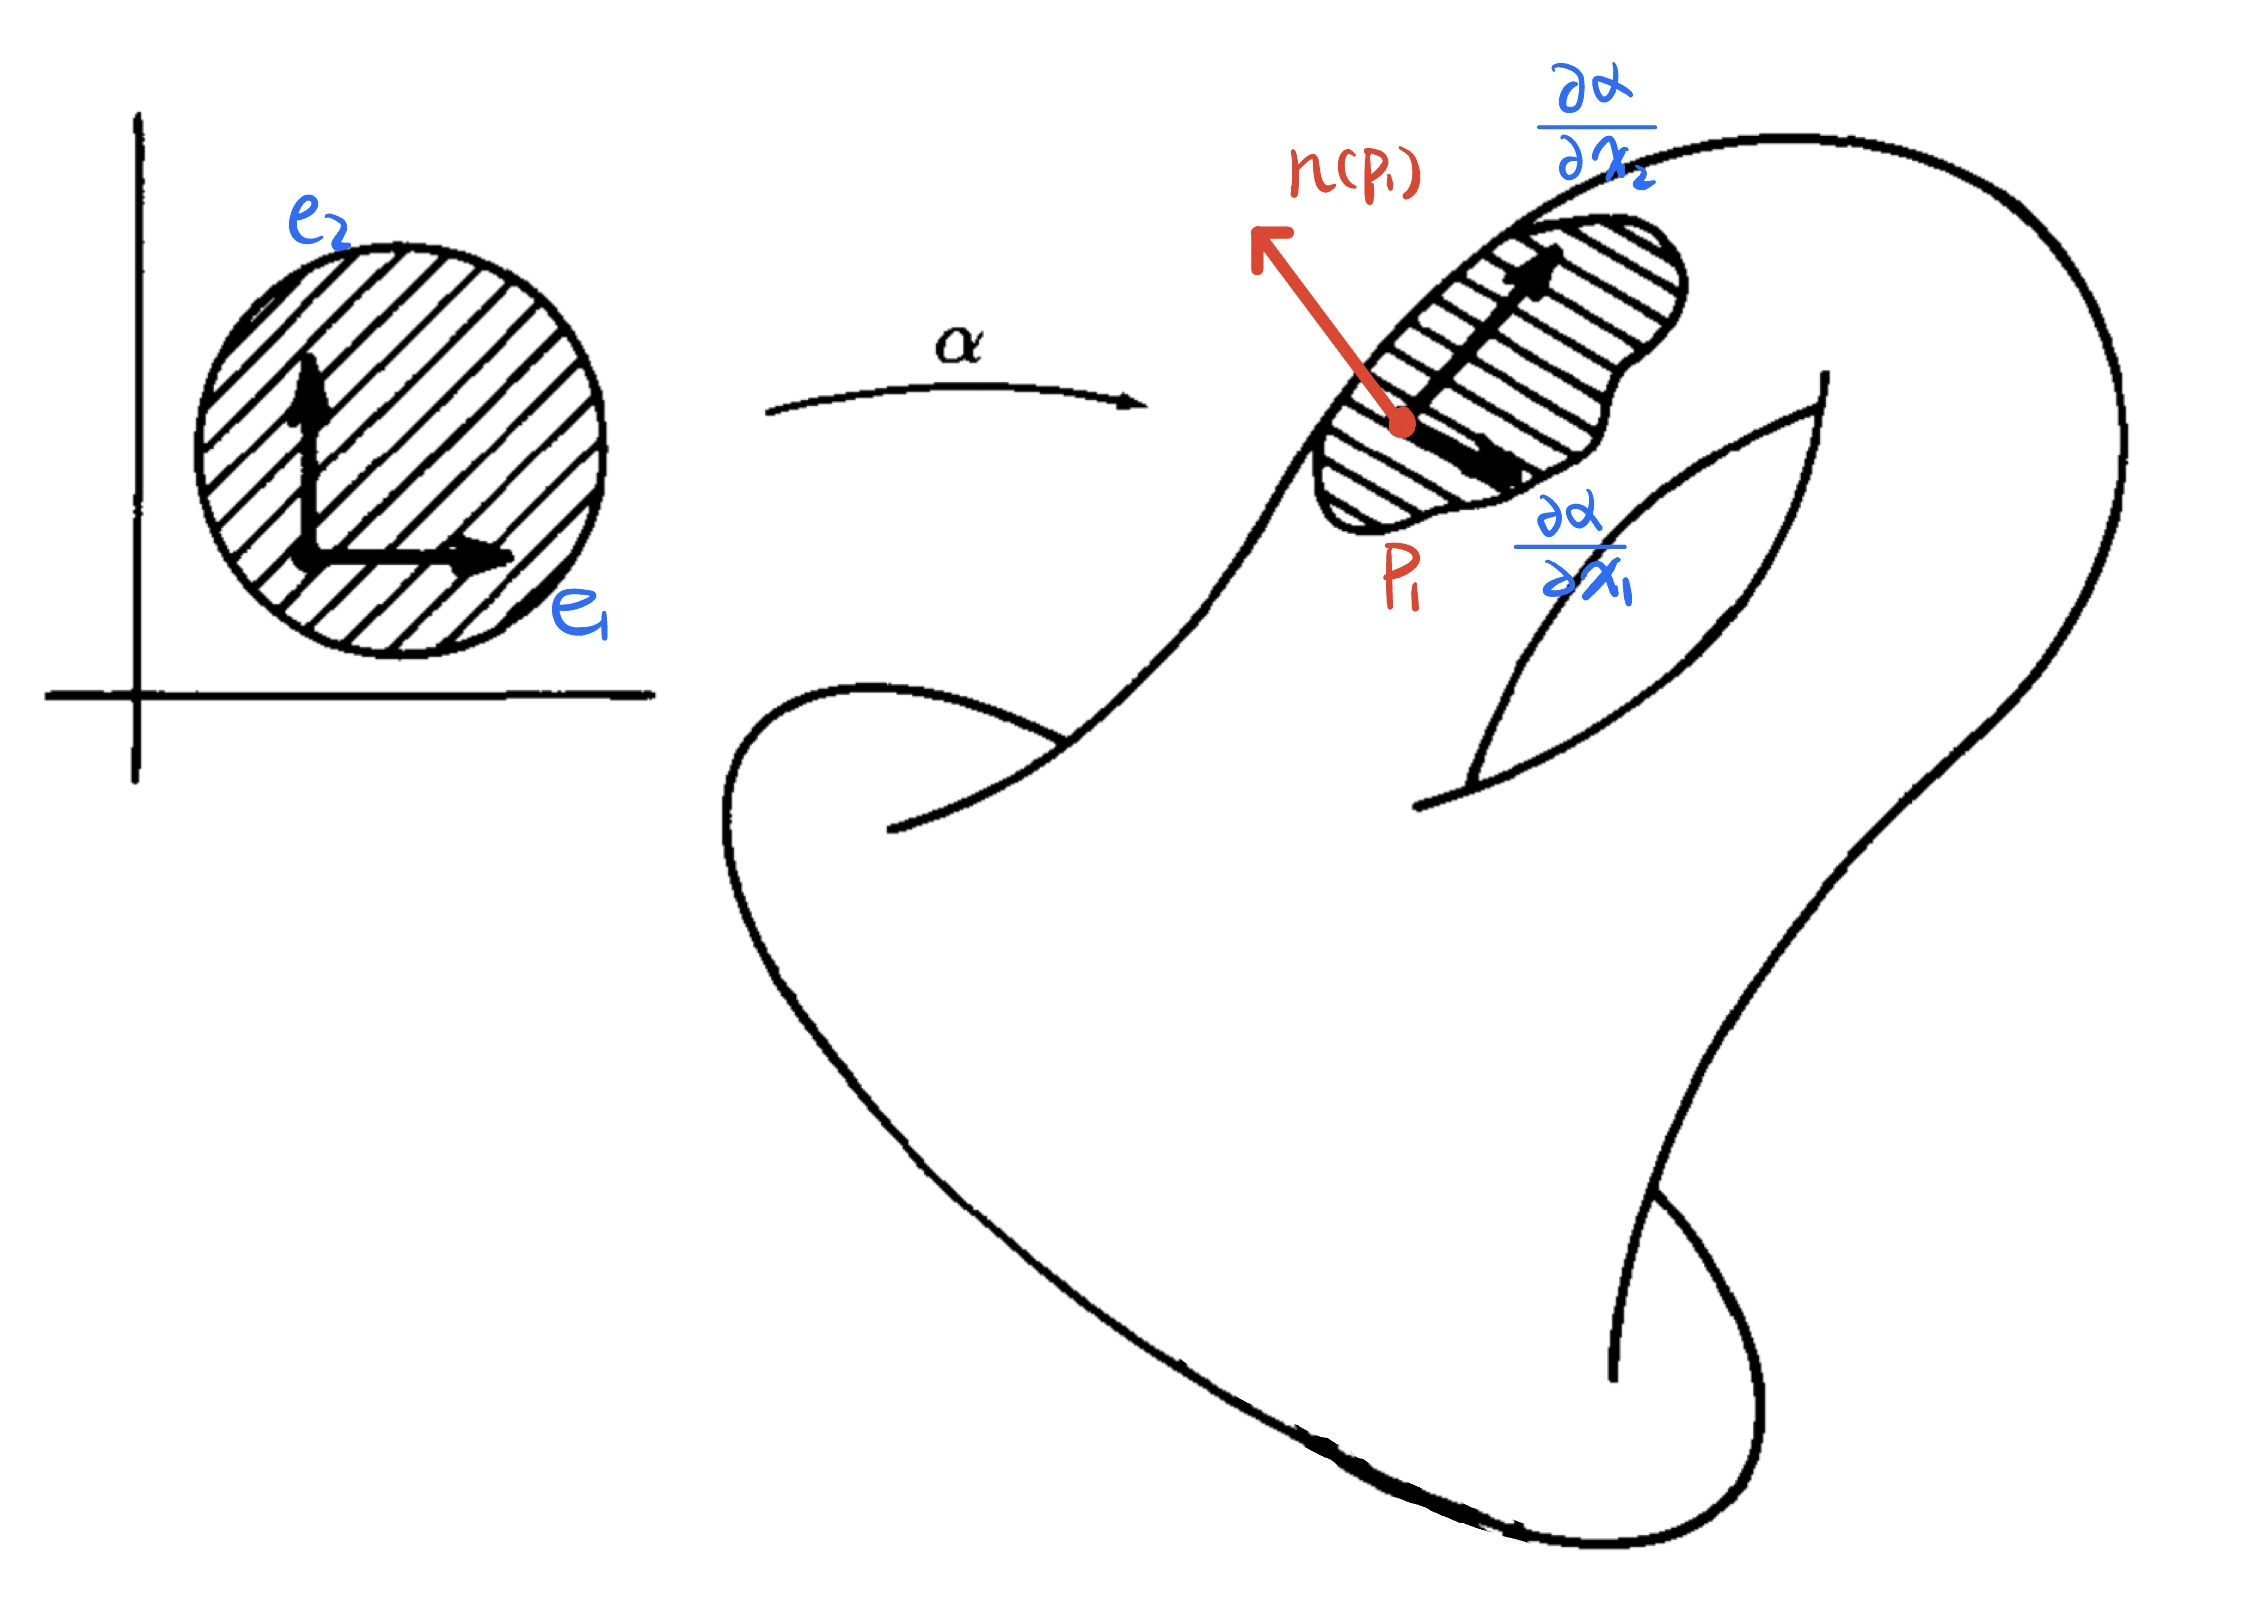
\includegraphics[scale=0.15]{images/IMG_0373.jpg}
    \end{figure}
    Consider the point $p_1$, the vector $n(p_1)$ is shown in the picture. Based on this orientation, for each point $p$, the vector $n(p)$ is pointing outward of the bell. 
    For the other orientation, $n(p)$ will pointing inside the bell. In this case, the two posiible orientations represent the outward of the manifold and the inward of the manifold.
    \item Consider $S^2$ in $\R^3$. Intuitively, this manifold also has two sides, inside and outside. Every point is like the above $p_1$.
    \item Now let us consider the famous Mobius band, which is a 2-manifold that can be embedded in $\R^3$. 
    \begin{figure}[H]
        \centering
        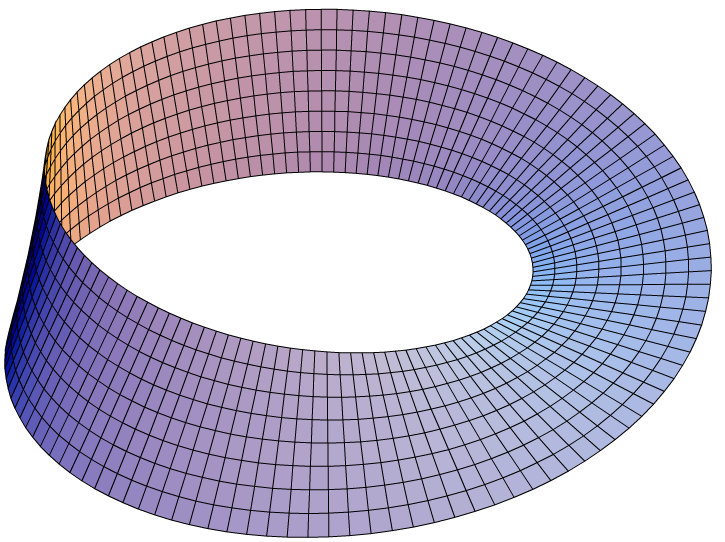
\includegraphics[scale=0.2]{images/Moebius_Surface_1_Display.png}
    \end{figure}
    This manifold is not orientable. Reason is simple, because all of us know that the mobius band only has one side! Rigorously, one can verify that we cannot have continuous unit normal vector field on the mobius band.
    Also from basic topology, we know that the Klein bottle is a 2-manifold that can be embedded in $\R^4$. Since it contains a copy of the mobius band, it is also not orientable. We will not give much details here. Everyone knows that the Klein bottle only has one side.
    \begin{figure}[H]
        \centering
        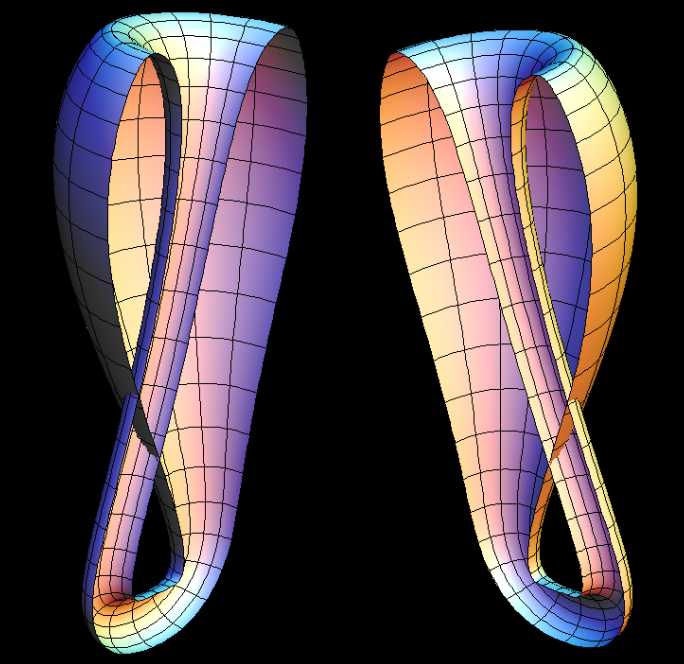
\includegraphics[scale=0.3]{images/kleinsymLR.png}
    \end{figure}
    Fun fact, we can stick two mobius bands along their edges to build a Klein bottle. This is a question on my topology final.
\end{itemize}

\begin{definition}
    Let $M$ be an n-manifold in $\R^n$. If $\alpha:U\longrightarrow V$ is a coordinate patch on $M$, then $D\alpha$ is an n by n matrix. 
    We define the \underline{nature orientation of $M$} to consist of all coordinate patches on $M$ for which $$\det(D\alpha)>0$$
    It is easy to see that two such patches overlap positively.
\end{definition}
\noindent\textbf{Remark}:
\begin{itemize}
    \item Consider $\alpha:U\longrightarrow V$, if $\det(D\alpha(x))<0$ for all $x\in U$, we need to apply the reflection map $$r(x_1,x_2,\cdots,x_n)=(-x_1,x_2,\cdots,x_n)$$
    Then $\alpha\circ r$ is the coordinate patch we want.
    Consider a 2-manifold in $\R^2$, the above can be shown in the picture
    \begin{figure}[H]
        \centering
        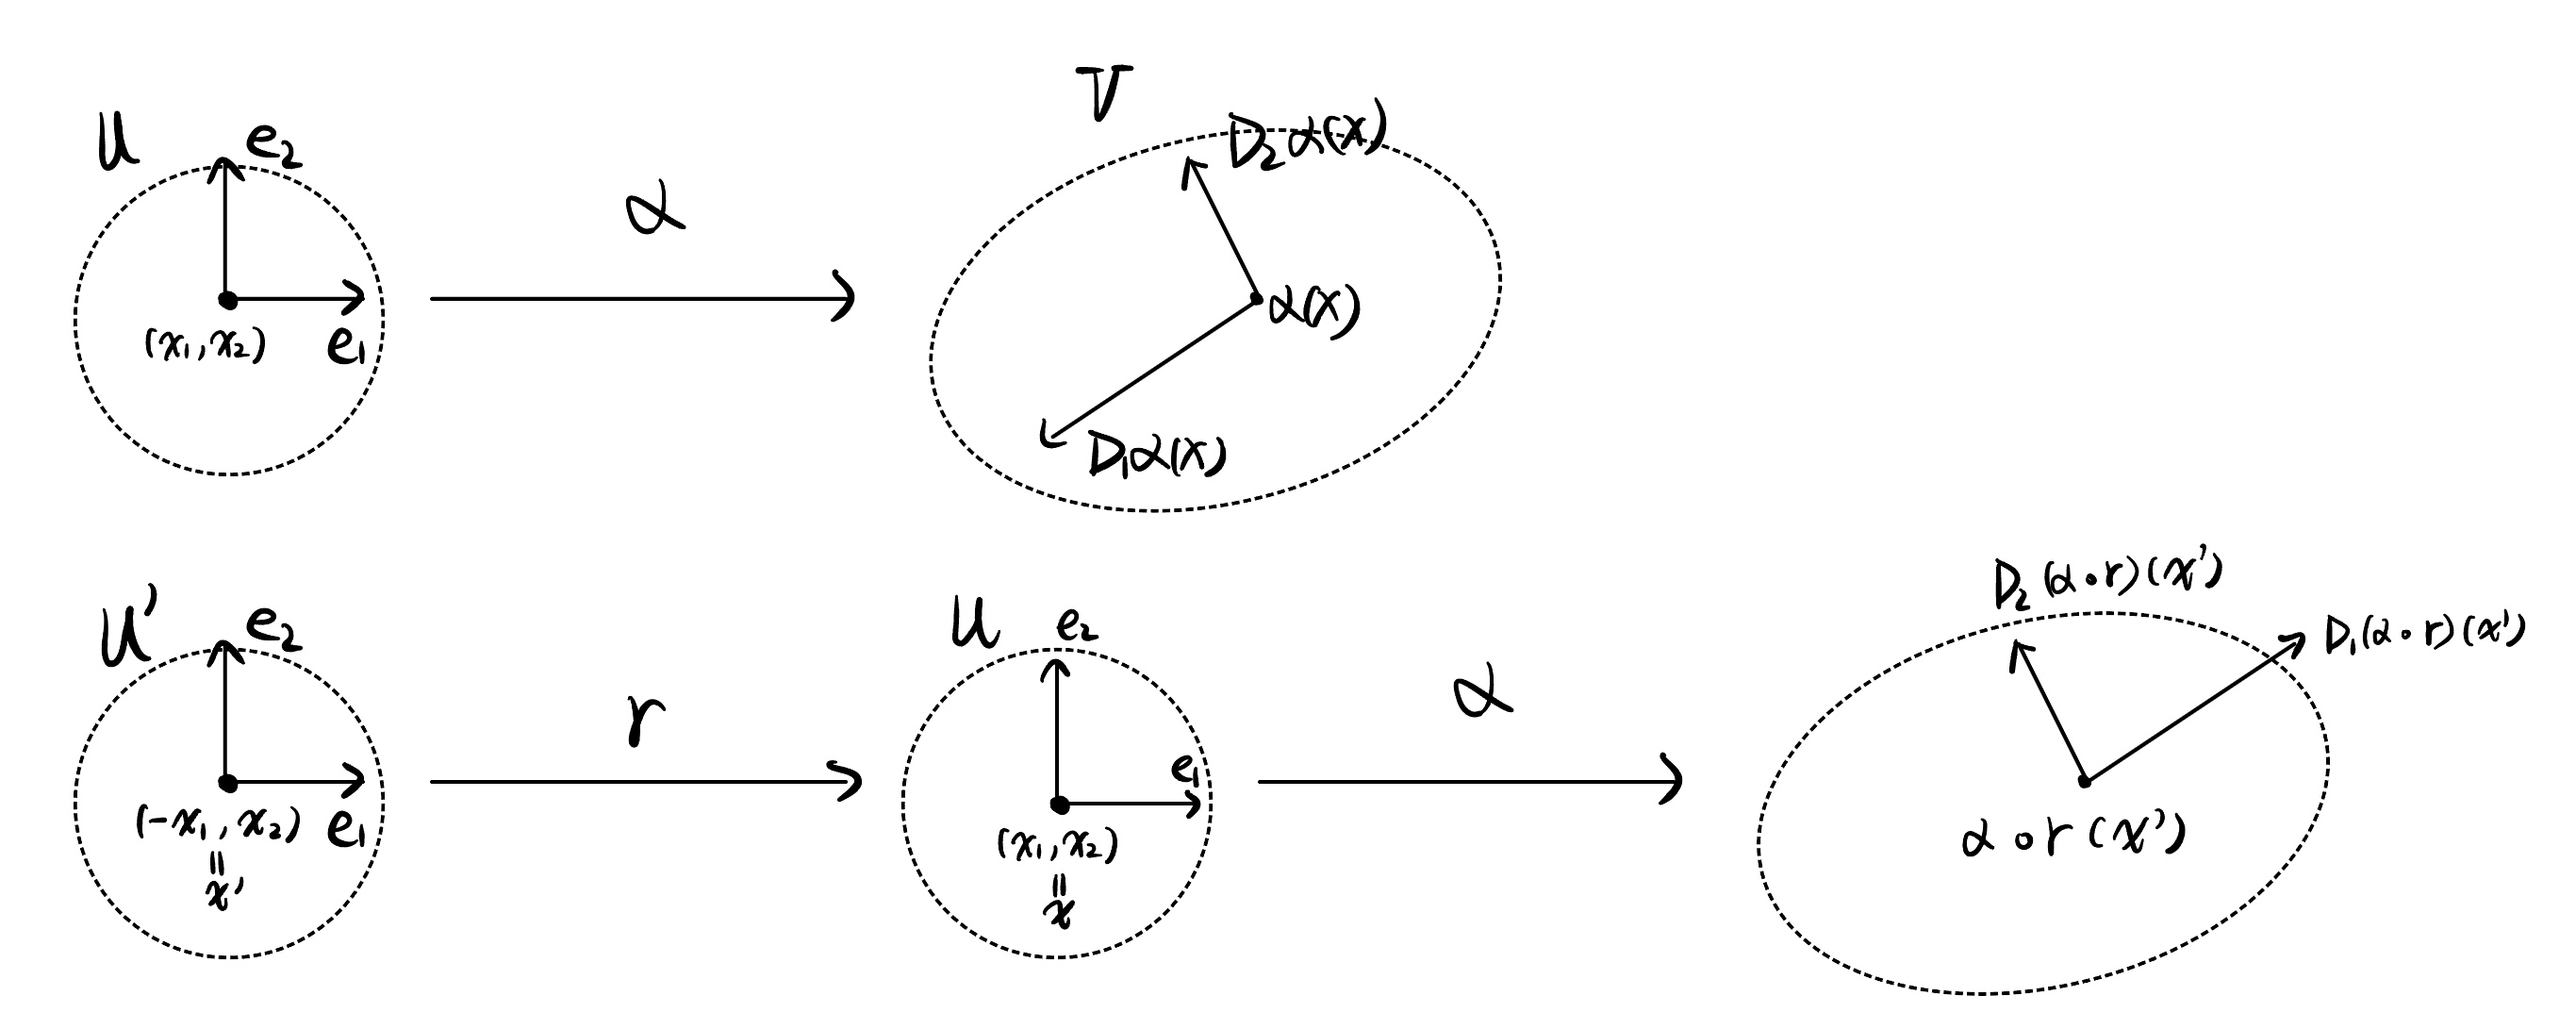
\includegraphics[scale=0.15]{images/IMG_0375.jpg}
    \end{figure}
    Notice that $$\alpha:U\longrightarrow V$$
    $$\alpha\circ r : U'\longrightarrow V$$
    where $U'$ is the open $U$ flipped along the y-axis. The above can be explained using the chain rule 
    \begin{equation*}
        \begin{split}
            D(\alpha\circ r)(x') &= D\alpha(r(x'))\cdot Dr(x')\\
            &= D\alpha(x)\cdot \begin{bmatrix}
                -1 & 0\\
                0 & 1
            \end{bmatrix}
        \end{split}
    \end{equation*}
\end{itemize}

\begin{definition}
    Let $M$ be an oriented k-manifold in $\R^n$. If $\alpha_i:U_i\longrightarrow V_i$ is a coordinate patch on $M$ belonging to the orientation of $M$. Let $\beta_i$ be the coordinate patches 
    $$\beta_i=\alpha_i\circ r: r(U_i)\longrightarrow V_i$$
    Then $\beta_i$ overaps $\alpha_i$ negatively, so it does not belong to the orientation of $M$. The coordinate pathches $\beta_i$ overlap each other positively, so they constitute another orientation of $M$. It is called the \underline{reverse or opposite} orientation to that specified by the coordinate pathches $\alpha_i$.
\end{definition}

\subsection{The Induced Orientation of $\partial M$}

\begin{theorem}
    Let $k>1$. If $M$ is an orientable k-manifold with non-empty boundary, then $\partial M$ is orientable.
\end{theorem}

\begin{definition}
    Let $M$ be an orientable k-manifold with non-empty boundary. Given an orientation of $M$, the corresponding \underline{induced orientation} of $\partial M$ is defined as follows: 
    \begin{itemize}
        \item If $k$ is even, it is the orientation obtaine by simply restriction coordinate patches belonging to the orientation of $M$.
        \item If $k$ is odd, it is the opposite of the orientation of $\partial M$ obtained in this way.
    \end{itemize}
\end{definition}

\noindent\textbf{Example}:
\begin{itemize}
    \item Consider a 3-manifold in $\R^3$ that is homeomorphic to the solid torus as shown in the picture. This is the case when $k=3$ which is odd. Consider the bottom point $p$ that is in the boundary. Let $$\alpha:U\longrightarrow V$$
    be the coordinate patch about $p$. $U$ is open in $\HH^3$.
    \begin{figure}[H]
        \centering
        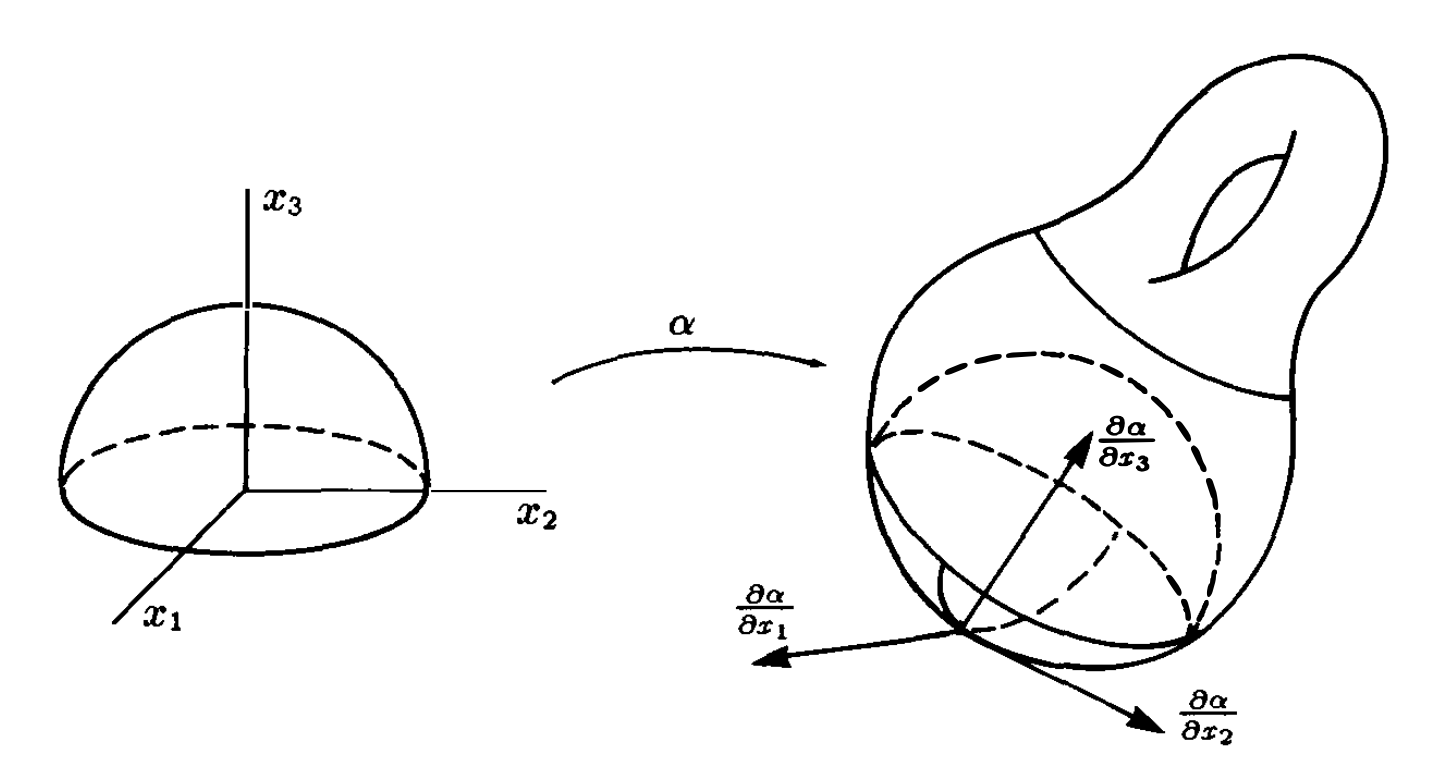
\includegraphics[scale=0.4]{images/Screenshot 2023-04-01 at 21.24.04.png}
    \end{figure}
    Now we restrict this coordinate patch to $\partial M$. $$\alpha|^{\partial M \cap V}:U'\longrightarrow V'$$
    where $U'\subset \R^2$ is the base of the half ball $U$ and $V'=\partial M\cap V$.
    $$\alpha|^{\partial M \cap V}(x_1,x_2)=\alpha(x_1,x_2,0)$$
    By the previous definition, we can assign a unit normal vector $n(p)$ such that $$(n(p),\frac{\partial \alpha|^{\partial M \cap V}}{\partial x_1},\frac{\partial \alpha|^{\partial M \cap V}}{\partial x_2})=(n(p),\frac{\partial \alpha}{\partial x_1},\frac{\partial \alpha}{\partial x_2})$$ is right-handed. But in here, we need the opposite, thus the normal field $$N(p)=(p;n(p))$$
    should have the property that $$(-n(p),\frac{\partial \alpha}{\partial x_1},\frac{\partial \alpha}{\partial x_2})$$ is right-handed. On the other hand, since $M$ is oriented naturally. It follows that 
    $$(\frac{\partial \alpha}{\partial x_3},\frac{\partial \alpha}{\partial x_1},\frac{\partial \alpha}{\partial x_2})$$ is right-handed. 
    It turns out that the orientation of $\partial M$ that corresponds to the unit normal field to $\partial M$ is pointing outwards.
    \item Now let us back to the weired bell that is a 2-manifold in $\R^3$. This is the case $k=2$ is even. 
    Consider the bottom point $p$ that is in the bouundary. Let $$\alpha:U\longrightarrow V$$
    be the coordinate patch about $p$. $U$ is open in $\HH^2$. 
    Let $N(p)=(p;n(p))$ be the unit normal field to $M$ corresponding to the orientation of $M$. 
    Let $T(p)=(p;\frac{D\alpha|^{\partial M\cap V}(t_0)}{\norm{D\alpha|^{\partial M\cap V}(t_0)}})$ be the unit tangent field to $\partial M$ corresponding to the induced orientation of $\partial M$. 
    The fun fact is that if you walk around $\partial M$ in the direction specified by $T$, with your head pointing in the direction specified by $N$, then the manifold $M$ is on your left.
    \begin{figure}[H]
        \centering
        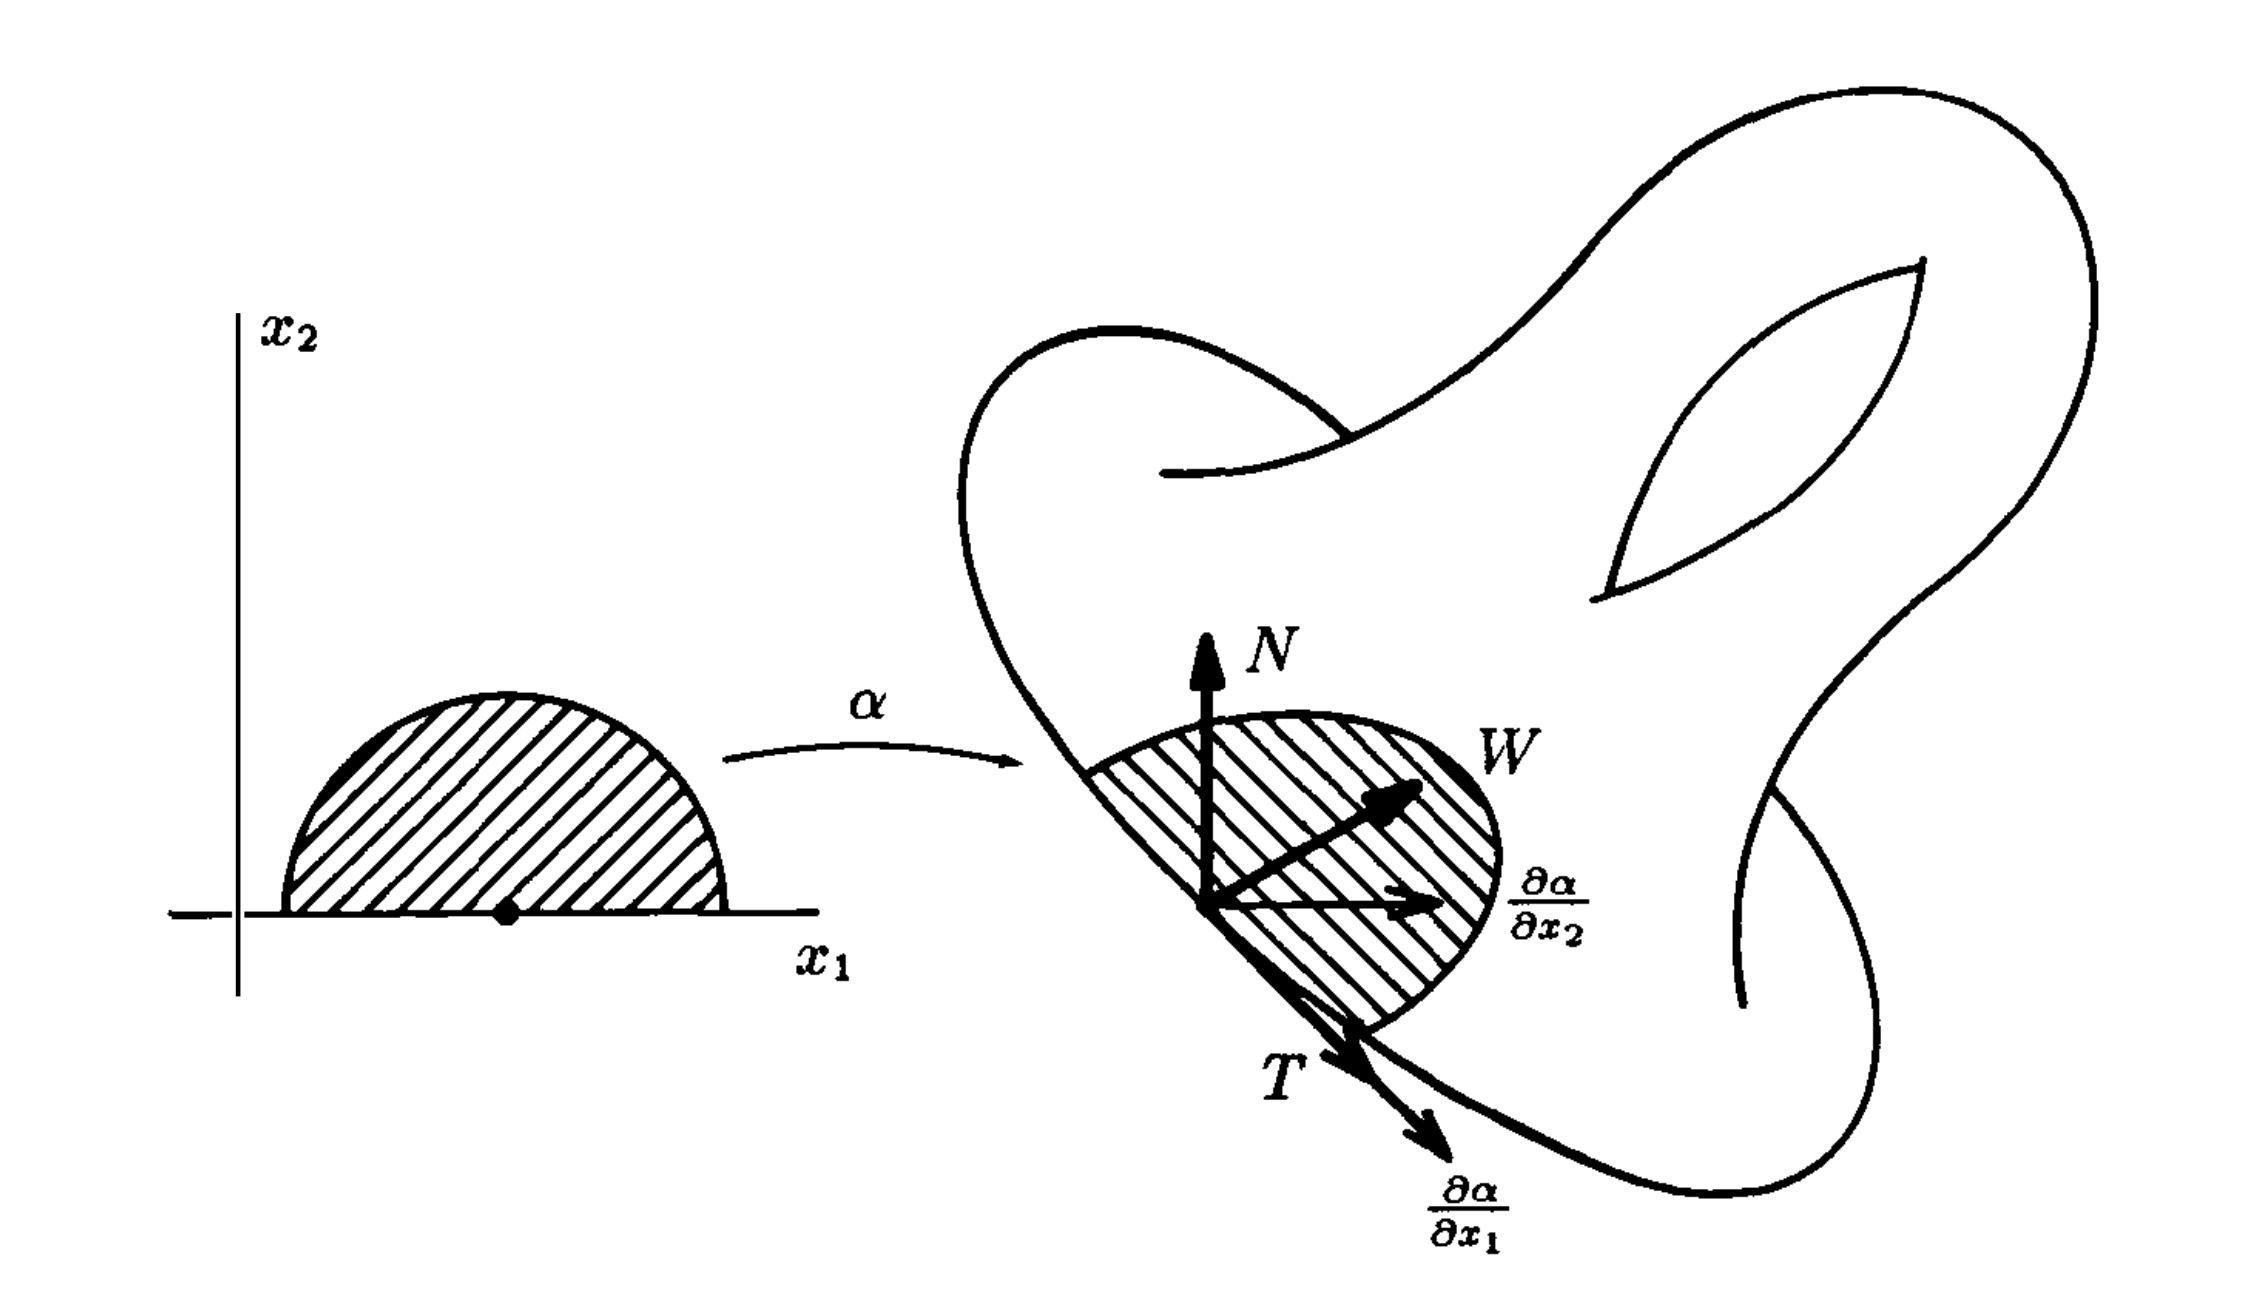
\includegraphics[scale=0.3]{images/Screenshot 2023-04-02 at 14.28.51.png}
    \end{figure}
    More precisely, let $W(p)=(p;w(p))$ that is perpendicular to both $N(p)$ and $T(p)$ such that $$(N(p),T(p),W(p))$$ is right-handed. Then $w(p)$ is tangent to $M$ at $p$ and points into $M$ from $\partial M$.
\end{itemize}

\section{Integrating Forms over Oriented Manifolds}

\begin{definition}
    Let $M$ be a compact oriented k-manifold in $\R^n$. Let $\omega$ be a k-form defined in an open set of $\R^n$ containing $M$. Let $C=M \cap supp(\omega)$. 
    Then $C$ is compact. Suppose there is a coordinate patch $\alpha:U \longrightarrow V$ on $M$ belonging to the orientation of $M$ such that $C\subset V$. By replacing $U$ by a smaller set if necessary, we can assume that $U$ is bounded. We define 
    the \underline{integral of $\omega$ over $M$} by the equation
    $$\int_M\omega=\int_{Int(U)}\alpha^*\omega$$
    Here $Int(U)=U$ is $U$ is open in $\R^k$, and $Int(U)=U\cap\HH^k$ if $U$ is open in $\HH^k$.
\end{definition}

\noindent\textbf{Remark}:
\begin{itemize}
    \item For the case $U$ is open in $\HH^k$, $\alpha$ can be extend to a $C^{\infty}$ map defined on $U'$ that is open in $\R^k$. So the form $\alpha^*\omega$ can be extended to a $C^{\infty}$ form on $U'$. This form can be written uniquely as $$\alpha^*\omega=h dx_1\wedge \cdots\wedge dx_k$$
    Therefore we have $$\int_{Int(U)}\alpha^*\omega=\int_{Int(U)}h$$
    \item The integral $\int_M\omega$ is well-defined, independent of the choice of the coordinate patch $\alpha$. Since now we choose $M$ to be an orineted manifold, we do not need to worry about the sign.
\end{itemize}

\begin{definition}
    Let $M$ be a compact oriented k-manifold in $\R^n$. we denote $-M$ as the manifold $M$ with the opposite orientation, then we have $$\int_{-M}\omega=-\int_M\omega$$
\end{definition}

\begin{definition}
    Let $M$ be a compact oriented k-manifold in $\R^n$. Let $\omega$ be a k-form defined in an open set of $\R^n$ containing $M$. Cover $M$ by coordinate pathches belonging to the orientation of $M$. 
    Then choose a partition of unity $\{\phi_1,\cdots,\phi_l\}$ on $M$ that is dominated by the coordinate patches on $M$. 
    We define the \underline{integral of $\omega$ over $M$} by the equation $$\int_M\omega=\sum_{i=1}^l[\int_M\phi_i\omega]$$
\end{definition}

\begin{theorem}[Linarity of integral of forms over oriented manifold]
    Let $M$ be a compact oriented mk-manifold in $\R^n$. Let $\omega$, $\eta$ be k-forms defined in anopen set of $\R^n$ containing $M$. Then $$\int_M(a\omega+b\eta)=a\int_M\omega +b\int_M\eta$$
    If $-M$ denotes $M$ with the opposite orientation, then $$\int_{-M}\omega=-\int_M\omega$$
\end{theorem}

\begin{theorem}
    Let $M$ be a compact oriented k-manifold in $\R^n$. Let $\omega$ be a k-form defined in an open set of $\R^n$ containing $M$. 
    Suppose $\alpha_i:A_i\longrightarrow M_i$ for $i=1,\cdots,N$, is a coordinate patch on $M$ belonging to the orientation of $M$, such that $A_i$ us open in $R^k$ and $M$ is the disjoint union of the open sets $M_1,\cdots,M_N$ of $M$ and a set $K$ of measure zero in $M$. Then $$\int_M\omega=\sum_{i=1}^N[\int_{A_i}\alpha^*\omega]$$
\end{theorem}

\section{A Geometric Interpretation of Forms and Integrals}

\begin{theorem}
    Let $W$ be a k-dimensional linear subspace of $\R^n$. 
    Let $(a_1,\cdots,a_k)$ be an orthonormal k-frame in $W$. 
    Let $f$ be an alternating k-tensor on $W$. 
    If $(x_1,\cdots,x_k)$ is an arbitrary k-tuple in $W$, then we have 
    $$f(x_1,\cdots,x_k)=\pm V(x_1,\cdots,x_k)f(a_1,\cdots,a_k)$$
    If the $x_i$ are independent and $(x_1,\cdots,x_k)$ and $(a_1,\cdots,a_k)$ belong to the same orientation of $W$, then the sign is $+$.
    If the $x_i$ are independent and $(x_1,\cdots,x_k)$ and $(a_1,\cdots,a_k)$ belong to the different orientation of $W$, then the sign is $-$. 
    If $x_i$ are dependent, then $V(x_1,\cdots,x_k)=0$ the sign does not matter. 
\end{theorem}

\begin{corollary}
    Let $(a_1,\cdots,a_k)$ and $(b_1,\cdots,b_k)$ be two orthonormal frames in $W$, then $$f(a_1,\cdots,a_k)=\pm f(b_1,\cdots,b_k)$$
    The sign depending on whether they belong to the same orientation of $W$ or not.
\end{corollary}

\noindent\textbf{Remark}:
\begin{itemize}
    \item Alternating tensors have geometric meanings, which can be seen in various contexts. Alternating tensors represent quantities that have a magnitude and orientation and are associated with area, volume, or higher-dimensional analogs.
    \item So given an alternating k-tensor on the vector space $W$, it tells us how to define a generalized volume.
\end{itemize}

\begin{definition}
    Let $M$ be a k-manifold in $\R^n$. If $M$ is oriented, then the tangent space to $M$ at $p$ has a natural induced orientation, defined as follows: 
    Choose a coordinate patch $\alpha:U\longrightarrow V$ belonging to the orientation of $M$ about $p$. Let $\alpha(x)=p$. The collection of all k-frames in $\mathcal{T}_p(M)$ of the form $$(\alpha_*(x;a_1),\cdots,\alpha_*(x;a_k))$$
    where $(a_1,\cdots,a_k)$ is a right-handed k-frame in $\R^n$. This collection is called the \underline{natural orientation} of $\mathcal{T}_p(M)$ induced by the orientation of $M$. 
    It is easy to show it is well-defined, independent of the choice of $\alpha$.
\end{definition}

\begin{theorem}
    Let $M$ be a compact oriented k-manifold in $\R^n$. Let $\omega$ be a k-form defined in an open set of $\R^n$ containing $M$. 
    Let $\lambda$ be a scalar function on $M$ defined by the equation $$\lambda(p)=\omega(p)((p;a_1),\cdots,(p;a_k))$$
    where $((p;a_1),\cdots,(p;a_k))$ is any orthonormal k-frame in the linear space $\mathcal{T}_p(M)$ belonging to its natrual orientation. Then $\lambda$ is continuous and $$\int_M\omega=\int_M\lambda \di V$$
\end{theorem}

\begin{theorem*}
    There exists a k-form $\omega_v$ defined in an open set about $M$ such that $\omega_v(p)$ on any orthonormal basis for $\mathcal{T}_p(M)$ belonging to its natural orientation is 1. 
    It is equivalent to say that $$\int_M\omega_v=\int_M\di V=v(M)$$
    The form $\omega_v$ is called a \underline{volume form for $M$}.
\end{theorem*}

\begin{corollary}
    Given any scalar function $\lambda$ on $M$, then we have $$\int_M\lambda\di V =\int_M\lambda\omega_v$$
\end{corollary}

\noindent\textbf{Remark}:
\begin{itemize}
    \item So back to the question how to understand differential forms? I think it tell us how to view the unit volume on the manifold.
\end{itemize}

\section{The Generalized Stokes' Theorem}

\begin{lemma}
    Let $k>1$. Let $\eta$ be a (k-1)-form defined in an open set $U$ of $\R^k$ containing the unit k-cube $I^k$. Assume that $\eta$ vanishes as all points of $Bd(I^k)$ except possibly at points of $Int(I^{k-1})\times 0$. Then 
    $$\int_{Int(I^k)}d\eta=(-1)^k\int_{Int(I^{k-1})}b^*\eta$$
    where $b:I^{k-1}\longrightarrow I^k$ is the map $$b(u_1,\cdots,u_{k-1})=(u_1,\cdots,u_{k-1},0)$$
\end{lemma}

\begin{theorem}[Stokes' Theorem for manifold of dimension $\geq 2$]
    Let $k>1$. Let $M$ be a compact oriented k-manifold in $\R^n$. 
    Give $\partial M$ the induced orientation if $\partial M$ is not empty. 
    Let $\omega$ be a (k-1)-form defiend in an open set of $\R6n$ containing $M$. Then 
    $$\int_Md\omega=\int_{\partial M}\omega$$
\end{theorem}

\begin{definition}
    Let $M$ be a 1-manifold in $\R^n$. Suppose there is a one-to-one map $\alpha:[a,b]\longrightarrow M$ of class $C^{\infty}$, carrying $[a,b]$ onto $M$ such that $D\alpha(t)\neq 0$ for all $t$. 
    Then we call $M$ a \underline{smooth arc} in $\R^n$. 
    If $M$ is oriented so that the coordinate patch $\alpha|_{(a,b)}$ belongs to the orientation, we say that $p$ is the \underline{initial point} of $M$ and $q$ 
    is the \underline{final point} of $M$.
    \begin{figure}[H]
        \centering
        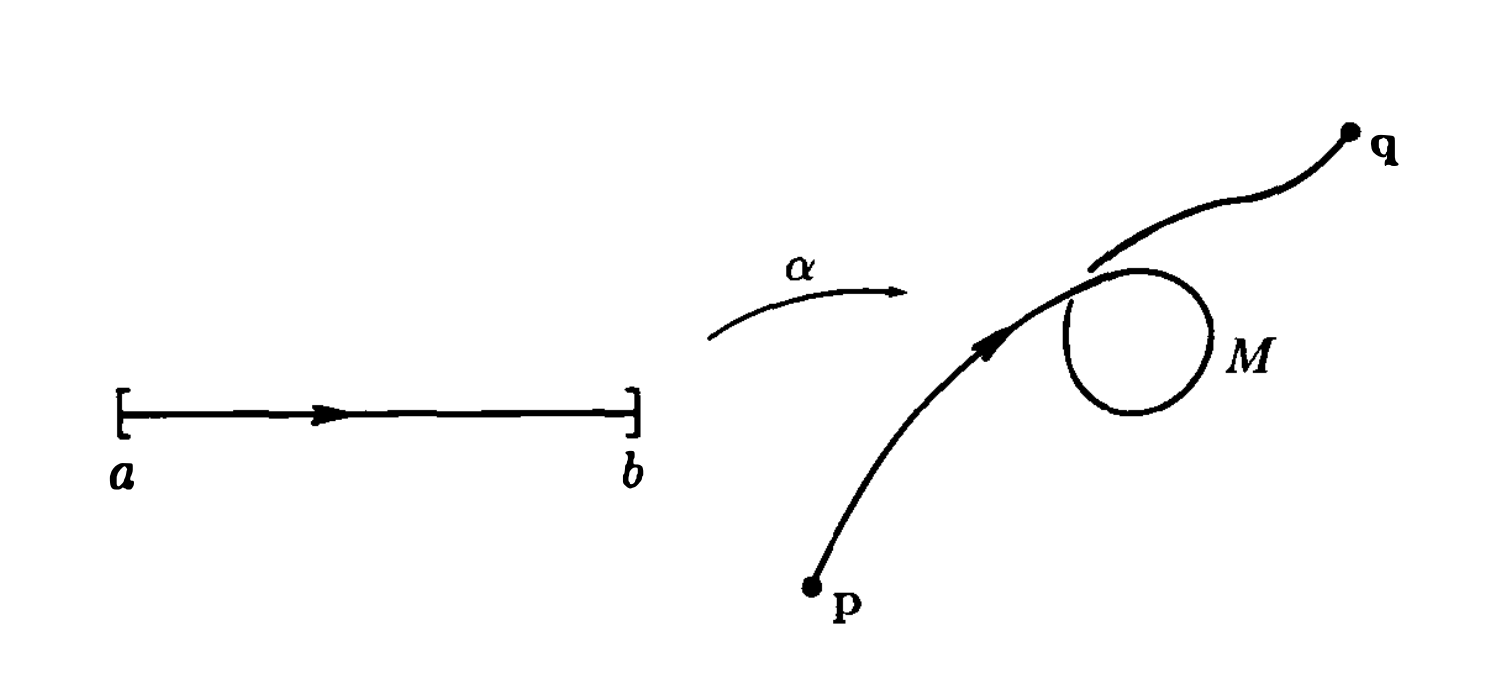
\includegraphics[scale=0.3]{images/Screenshot 2023-04-02 at 16.28.02.png}
    \end{figure}
\end{definition}

\begin{lemma}
    Let $M$ be a 1-manifold in $\R^n$. Let $f$ be a 0-form defined in an open set about $M$. If $M$ is an arc with initial point $p$ and final point $q$, then $$\int_Mdf=f(q)-f(p)$$
\end{lemma}

\begin{definition}
    A compact 0-manifold $N$ in $\R^n$ is a finite collection of points $\{x_1,\cdots,x_m\}$ of $\R^n$. 
    We defien an \underline{orientation of $N$} to be a function $$\epsilon:N\longrightarrow \{-1,1\}$$
\end{definition}

\begin{definition}
    If $M$ is an oriented 1-manifold in $\R^n$ with nnon-empty boundary, we define the \underline{induced orientation} of $\partial M$ by setting:
    \begin{itemize}
        \item If there is a coordinate patch $\alpha:U\longrightarrow V$ about $p\in\partial M$ belonging to the orientation of $M$ with $U$ open in $\HH^1$, we set $\epsilon(p)=-1$
        \item If there is a coordinate patch $\alpha:U\longrightarrow V$ about $p\in\partial M$ belonging to the orientation of $M$ with $U$ open in $\mathbb{L}^1$, we set $\epsilon(p)=1$
    \end{itemize}
    \begin{figure}[H]
        \centering
        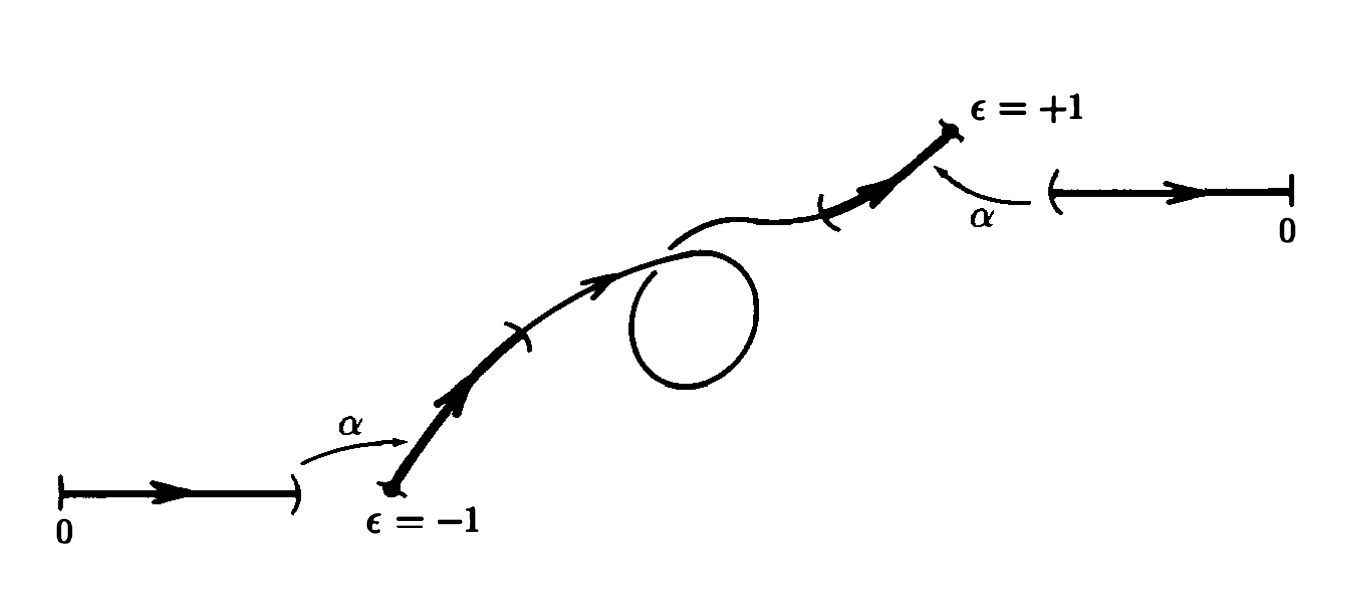
\includegraphics[scale=0.4]{images/Screenshot 2023-04-02 at 16.36.44.png}
    \end{figure}
\end{definition}

\begin{definition}
    let $f$ be a 0-form defined in an open set of $\R^n$ containing $N$, we define the \underline{integral of $f$ over oriented $N$} by $$\int_Nf=\sum_{i=1}^m\epsilon(x_i)f(x_i)$$
\end{definition}

\begin{theorem}{Stokes theorem for 1-manifold}
    Let $M$ be a compact oriented 1-manifold in $\R^n$. Give $\partial M$ the induced orientation if $\partial M$ is not empty. Let $f$ be a 0-form defined in an open set of $\R^n$ containing $M$. Then $$\int_Mdf=\int_{\partial M}f$$
\end{theorem}
\noindent\textbf{Remark}:
\begin{itemize}
    \item Recall the fundamental theorem of calculus, it is just the case when $n-1$ for this theorem!
\end{itemize}